\part{Pour aller plus loin\textellipsis}

\begin{exercice}[Continuité (suite)]
La fonction $u : \mathbb{R} \to \mathbb{R}$ de l'Exercice \ref{ex:weird_function} admet un prolongement par continuité en $x = 0$, car la limite existe et vaut $0$. Cependant, elle ne peut pas être prolongée sur tout $\mathbb{R}$ en une fonction $\tilde{u}$ continue, car la limite diverge en $x = \pm 1$. Ainsi, un tel $\tilde{u}$ n'existe pas.
\end{exercice}

\begin{exercice}[Rencontres du troisième type (d'extremum)]
Soit $f : \mathbb{R} \to \mathbb{R}$ définie par $f(x) = \sin(x)^3$.

\begin{enumerate}
    \item Calculer $f'(x)$.
    
    En utilisant les propriétés de la dérivée on obtient :
    \begin{align*}
        f'(x) &= \left( \sin(x)^3 \right)' & \textrm{ de la forme } \big( f(g(x)) \big)' = g'(x) f'(g(x)) \\
        &= \cos(x) \left( 3 \sin(x)^2 \right)
    \end{align*}
    Donc $f'(x) = 3 \sin(x)^2 \cos(x)$
    
    \item Trouver le(s) point(s) telle que $f'(x) = 0$.
    \begin{align*}
        f'(x) = 0 & \iff 3 \sin(x)^2 \cos(x) = 0 \\
                  & \iff \sin(x) = 0 \textrm{ ou } \cos(x) = 0 \\
                  & \iff x = k \frac{\pi}{2}, \ k \in \mathbb{Z} 
    \end{align*}
    
    \item Parmi ce(s) point(s), trouver les minimums et les maximums.
    
    Pour déterminer s'il s'agit de minimum ou de maximum on étudie le signe de la dérivée. Notons que comme $\sin(x)^2 \geq 0$, le signe de $f'$ dépend uniquement du signe de $\cos(x)$. De plus, comme $f'$ est $2\pi$-périodique, il nous suffit d'étudier son comportement sur l'intervalle $[0, 2\pi]$ pour en déduire son comportement général.
    
    \begin{table}[H]
        \centering
        \begin{tikzpicture}
            \tkzTabInit{$x$/1, $f'(x)$/1}{$0$, $\frac{\pi}{2}$, $\pi$, $\frac{3\pi}{2}$, $2\pi$}
            \tkzTabLine{z, + , z, -, z, -, z, +, z}
        \end{tikzpicture}
        \caption{Tableau de signe de $f'(x) = 3 \sin(x)^2 \cos(x)$}
        \label{tab:signe_derivee}
    \end{table}
    
    On distingue alors les 3 cas de zéros~:
    \begin{itemize}
        \item \emph{Cas n°1}~: Extremum en $x = \frac{\pi}{2} + 2k\pi$
        
        On peux voir sur le Tableau $\ref{tab:signe_derivee}$ qu'au alentour de $\frac{\pi}{2} + 2k\pi$, la dérivée change de signe, passant de positif à négatif. Ainsi les extremums de la forme $x = \frac{\pi}{2} + 2k\pi$ sont des maximums.
        
        \item \emph{Cas n°2}~: Extremum en $x = \frac{3\pi}{2} + 2k\pi$
        
        De même, on peux voir qu'au alentour de $\frac{3\pi}{2} + 2k\pi$, la dérivée passe d'un signe négatif à positif. Ainsi, les extremums de la forme $x = \frac{3\pi}{2} + 2k\pi$ sont des minimums.

        \item \emph{Cas n°3}~: Extremum à $x = k \pi$

        Étrangement, le signe au alentours de $x = k \pi$ semble ne pas changer. Ainsi, bien que la dérivé soit nulle, \emph{il ne s'agit ni d'un maximum, ni d'un minimum} !
    \end{itemize}
    
    \item
    Soit $\sign : \mathbb{R} \to \mathbb{R}$ telle que
    \[
    \sign(x) = \begin{cases}
    1 & \textrm{si } x > 0 \\
    0 & \textrm{si } x = 0 \\
    -1 & \textrm{si } x < 0
    \end{cases}
    \]
    
    Évaluer $\displaystyle \lim_{x \to 0^+} \sign(f'(x))$ et $\displaystyle \lim_{x \to 0^-} \sign(f'(x))$.
    
    \medskip
    
    On a par le tableau ci-dessus que
    \[
    \lim_{x \to 0^+} \sign(f'(x)) = 1 \quad \textrm{et} \quad \lim_{x \to 0^-} \sign(f'(x)) = \lim_{x \to 2\pi^-} \sign(f'(x)) = 1
    \]
    
    \item On peux voir que la fonction $f'(x)$ est positive au alentour de $x = 0$ (comme le démontre le point 4). Bien que $f'(0) = 0$, la dérivée reste positive donc il ne s'agit donc pas d'un minimum où d'un maximum. Peut-on se représenter quel est le problème ici ?
    
    La dérivée est une mesure de la croissance~: comme $f'(0) = 0$, au point $0$ la courbe ne monte ni ne descend. Pourtant, aux alentours de ce point la dérivé est positive et donc la fonction augmente. Ainsi la fonction admet une sorte de "plateau" en $x = 0$, car elle arrête momentanément de croître, ce qui pourrait nous tromper à penser que c'est un extremum si l'on oublie de vérifier que la dérivée change bien de signe.
    
    \begin{figure}[H]
        \centering
        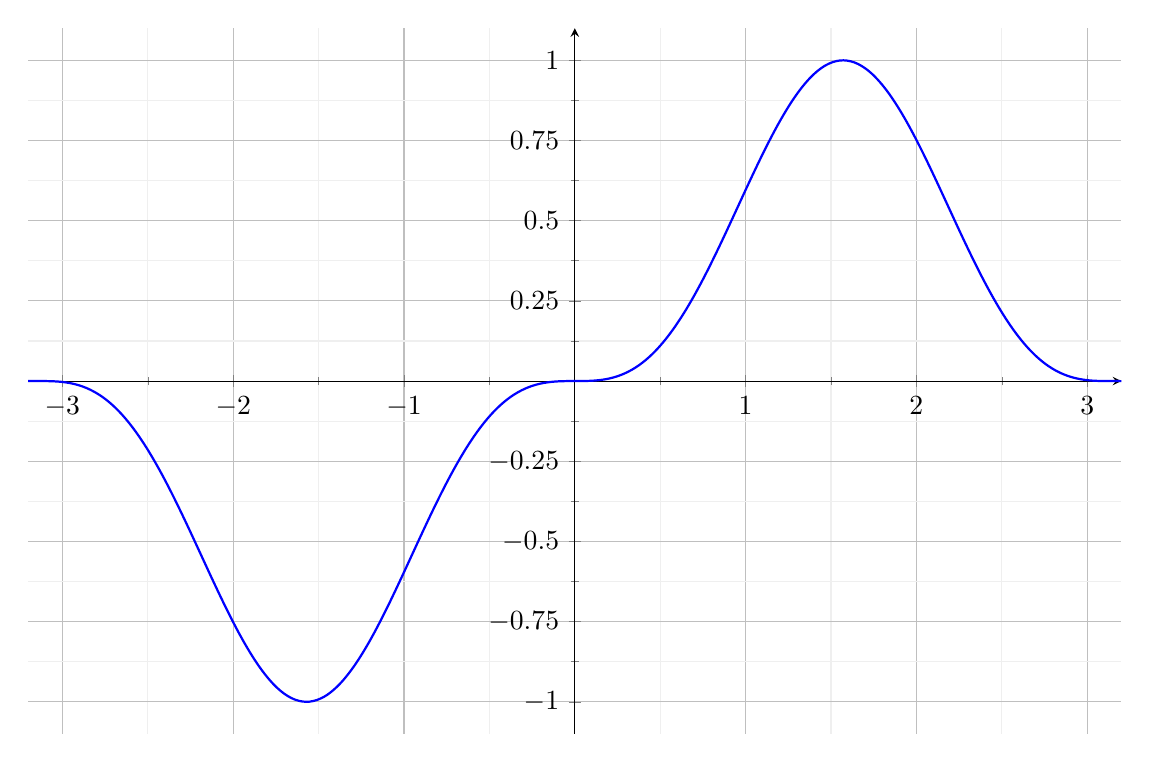
\begin{tikzpicture}
            \begin{axis}[
                xmin = -3.2, xmax = 3.2,
                ymin = -1.1, ymax = 1.1,
                xtick distance = 1,
                ytick distance = 0.25,
                grid = both,
                minor tick num = 1,
                major grid style = {lightgray},
                minor grid style = {lightgray!25},
                width = 440,
                height = 300,
                legend cell align = {left},
                legend pos = north west,
                axis lines=middle,
                trig format plots=rad
            ]
                
            \addplot[
                domain = -3.2:3.2,
                samples = 300,
                smooth,
                thick,
                blue,
            ] {sin(x)^3};
                
            \end{axis}
        \end{tikzpicture}
        \caption{Graphe de $f(x) = \sin(x)^3$ sur $[-\pi, \pi]$}
        \label{fig:sin_cubed}
    \end{figure}
\end{enumerate}
\end{exercice}

\begin{exercice}[Tout mettre ensemble]
Pour quelles valeurs de $a, b \in \mathbb{R}$ la fonction $f : \mathbb{R} \to \mathbb{R}$ définie par
\[
f(x) = \begin{cases}
ax + 5 & \textrm{si } x \leq 2 \\
\sqrt{bx^2 + 1} & \textrm{si } x > 2
\end{cases}
\]
est-elle dérivable en $2$ ?

Premièrement, pour que $f$ soit dérivable en $2$, il faut nécessairement que $f$ soit continue en $2$ (cf. cours). Ainsi, on commence par étudier les limites à droite et à gauche~:
\[
\lim_{x \to 2^-} ax = 2a + 5 \quad \textrm{et} \quad \lim_{x \to 2^+} \sqrt{bx^2 + 1} = \sqrt{4b + 1}
\]
Pour que $f$ soit continue, l'équation $2a + 5 = \sqrt{4b + 1} = f(2)$ doit être vérifiée, ce qui nous donne
\[
(2a + 5)^2 = 4b + 1
\]
De plus, pour que $f$ soit dérivable, on doit avoir
\[
\lim_{h \to 0^-} \frac{f(2+h)-f(2)}{h} = \lim_{h \to 0^+} \frac{f(2+h)-f(2)}{h}
\]
où les deux limites sont obtenues par la définition de $f$~: à gauche, on obtient
\[
\lim_{h \to 0^-} \frac{a(2 + h) + 5 - (2a + 5)}{h} = \lim_{h \to 0^-} \frac{ah}{h} = a
\]
tandis qu'à droite on obtient
\begin{align*}
\lim_{h \to 0^+} \frac{\sqrt{b(2 + h)^2 + 1} - (2a + 5)}{h} & = \lim_{h \to 0^+} \frac{\sqrt{b(2 + h)^2 + 1} - (2a + 5)}{h} \frac{\sqrt{b(2 + h)^2 + 1} + (2a + 5)}{\sqrt{b(2 + h)^2 + 1} + (2a + 5)} \\
& = \lim_{h \to 0^+} \frac{b(2+h)^2 + 1 - (2a + 5)^2}{h (\sqrt{b(2 + h)^2 + 1} + 2a + 5)}
\end{align*}
En subsistuant $(2a + 5)^2 = 4b + 1$, on a
\begin{align*}
\lim_{h \to 0^+} \frac{b(2+h)^2 - 4b}{h (\sqrt{b(2 + h)^2 + 1} + \sqrt{4b + 1})} & = \lim_{h \to 0^+} \frac{b(4 + 4h + h^2) - 4b}{h (\sqrt{b(2 + h)^2 + 1} + \sqrt{4b + 1})} \\
& = \lim_{h \to 0^+} \frac{(4 + h)b}{\sqrt{b(2 + h)^2 + 1} + \sqrt{4b + 1}} \\
& = \frac{4b}{2\sqrt{4b + 1}} \\
& = \frac{2b}{\sqrt{4b + 1}}
\end{align*}
Notez que c'est le même résultat que si l'on avait dérivé $\sqrt{bx^2 + 1}$ par nos propriétés, évalué en $x = 2$. C'est en effet toujours le cas, et on peut se passer du calcul des limites ci-dessus en calculant les dérivées de part et d'autre de $2$, et en les mettant en égalité.
Cela peut accélérer le processus, notamment sous la contrainte du temps en examen.

\medskip
\noindent Le système que l'on doit résoudre est alors
\[
\begin{cases}
2a + 5 & = \sqrt{4b + 1} \\
a & = \frac{2b}{\sqrt{4b + 1}}
\end{cases}
\]
d'où l'on trouve
\[
\frac{4b}{\sqrt{4b + 1}} + 5 = \sqrt{4b + 1}
\]
Cette équation peut être résolue de différentes manières~; en isolant le terme constant, on a
\[
5 = \frac{4b + 1}{\sqrt{4b + 1}} - \frac{4b}{\sqrt{4b + 1}} = \frac{1}{\sqrt{4b + 1}}
\]
d'où l'on obtient $\sqrt{4b + 1} = \frac{1}{5} \implies 4b + 1 = \frac{1}{25}$, i.e. $b = -\frac{6}{25}$. En substituant la valeur de $b$ dans l'équation $a = \frac{2b}{\sqrt{4b + 1}}$, on obtient
\[
a = \frac{-\frac{12}{25}}{\frac{1}{5}} = -\frac{12}{5}
\]
Ainsi, $f$ est dérivable en $2$ si et seulement si $a = -\frac{12}{5}$ et $b = -\frac{6}{25}$. Ces valeurs sont uniques puisque ce sont les seules solutions du système d'équations.
\end{exercice}